\section{Genetic team composition and level of selection in the evolution of cooperation \cite{waibel2009genetic}}

\begin{frame}{Problem Description}

\begin{figure}
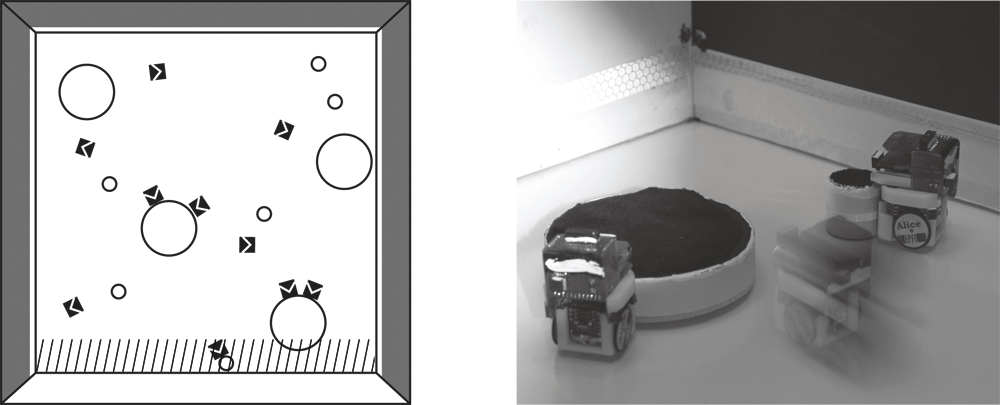
\includegraphics[width=\textwidth]{waibel-fig-3}
\vspace{1ex}
\caption{
Figure 3 from \cite{waibel2009genetic}.
}
\end{figure}

\end{frame}

\begin{frame}{Treatments}

\begin{figure}
\begin{columns}
\begin{column}{0.7\textwidth}
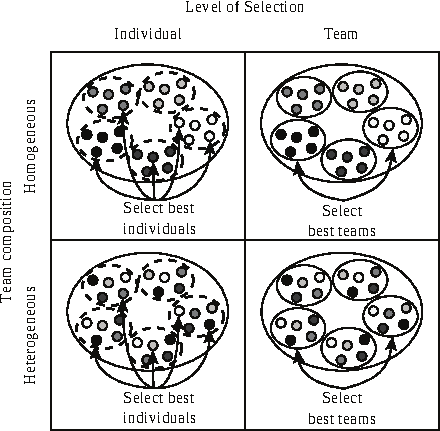
\includegraphics[width=\textwidth]{waibel-fig-2}
\end{column}
\begin{column}{0.3\textwidth}
\caption{
Figure 2 from \cite{waibel2009genetic}.
}
\end{column}
\end{columns}
\end{figure}

\end{frame}

\begin{frame}{Treatments}

  Task 1—Individual Foraging: The arena contained
  6 small tokens, each of which awarded 1 fitness point to the
  foraging robot. This task did not require cooperation, because
  a single agent was sufficient to transport a small token.
  2) Task 2—Cooperative Foraging: The arena contained
  four large tokens, which each awarded 1 fitness point to each
  team member, irrespective of its participation in the token
  foraging. This corresponded to a situation where the individual
  contributions to team performance were not known, i.e., a
  situation with credit assignment problems [70], [71], which is
  the case for many cooperative multiagent tasks [72]. This task
  required cooperation because it could not be accomplished by
  a single agent.
  3) Task 3—Altruistic Cooperative Foraging: The arena
  contained six small and four large tokens. Small tokens each
  awarded one fitness point to the foraging robot and large
  tokens each awarded one fitness point to each team member,
  irrespective of their participation in the token foraging. In this
  task cooperation was costly for individuals, because individu-
  als that did not cooperate always had higher fitness than their
  cooperating team mates. This meant that cooperators suffered
  a relative individual fitness cost and therefore this task required
  altruistic cooperation [6

\end{frame}

\begin{frame}{Results}

\begin{figure}
\begin{columns}
\begin{column}{0.7\textwidth}
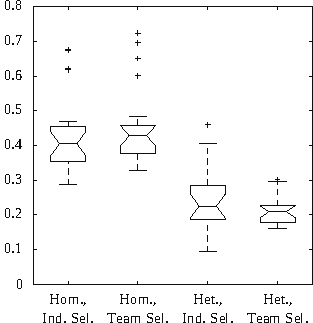
\includegraphics[width=\textwidth]{waibel-fig-9-b}
\end{column}
\begin{column}{0.3\textwidth}
\caption{
Right column of Figure 9 from \cite{waibel2009genetic}.
}
\end{column}
\end{columns}
\end{figure}

\end{frame}

\begin{frame}{Results}


\begin{figure}
\begin{columns}
\begin{column}{0.7\textwidth}
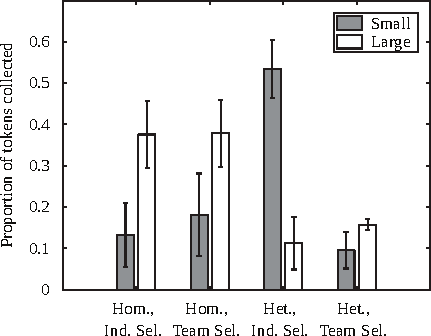
\includegraphics[width=\textwidth]{waibel-fig-10}
\end{column}
\begin{column}{0.3\textwidth}
\caption{
Figure 10 from \cite{waibel2009genetic}.
}
\end{column}
\end{columns}
\end{figure}

\end{frame}

\begin{frame}{Results}

\begin{figure}
\begin{columns}
\begin{column}{0.8\textwidth}
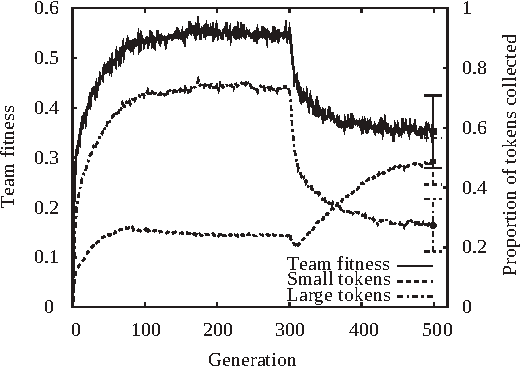
\includegraphics[width=\textwidth]{waibel-fig-12}
\end{column}
\begin{column}{0.2\textwidth}
\caption{
Figure 12 from \cite{waibel2009genetic}.
}
\end{column}
\end{columns}
\end{figure}

\end{frame}

\begin{frame}{Discussion}

\end{frame}
